\section{Systematic errors}
\label{sec: systematics}

Several systematic errors contribute to the overall uncertainty on the branchning fractions. We consider the most significant ones:

\begin{itemize}

\item Particle identification

\item Signal and background models

\item Determination of the selection efficiency with MC

\item The relative trigger efficiency

\item The relative tracking efficiency

\item MC statistics

\item BDTG efficiency

\end{itemize} 

The particle identification (PID) efficiency is determined using PIDcalib in bins of pseudorapidity $\eta$ and transverse momentum $\pt$ of each $\Bs$ candidate. 
To estimate the systematic uncertainty, the baseline binning scheme was changed to alternative $\eta$ and $\pt$ bins. 
Tab. \ref{tab: PIDbinning} summarizes the tested binning schemes and the observed effect on $\epsilon^{pid}$. 

\begin{table}[h]
\centering
\begin{tabular}{l l l l}
 & baseline & alternative 1 & alternative 2\\
\hline
$\ptot$ bins [$\mevc$] & \scriptsize 3000-9300-15600-19000&\scriptsize 0-10000-20000-30000-40000&\scriptsize 1000-8450-15900-23350\\&\scriptsize-24400-29800-35200-40600&\scriptsize-50000-60000-70000-80000-90000&\scriptsize-30800-38250-45700-53150\\&\scriptsize-46000-51400-56800-62200&\scriptsize-100000&\scriptsize-60600-68050-75500-82950\\&\scriptsize-67600-73000-78400-83800&&\scriptsize-90400-97850-105300-112750\\&\scriptsize-89200-94600-100000&&\scriptsize-120200-127650-135100-142550\\&&&\scriptsize-150000\normalsize\\
\hline
$\eta$ bins  &\scriptsize 1.5-2.375-3.25-4.125-5 &\scriptsize 2-2.3-2.6-2.9-3.2-3.5-3.8-4.1-4.4-4.7-5 & \scriptsize 1.5-2.2-3.1-4-5\normalsize\\
\hline \hline
$\Delta\epsilon^{pid}$      & - & 0.4 $\%$ & 0.15 $\%$\\
\end{tabular}
\caption{Summary of considered binning schemes for the determination of the PID efficiency using PIDCalib.}
\label{tab: PIDbinning}
\end{table}


The maximum change in the PID efficiency due to the binning scheme is observed to be 0.4 $\%$. \newline
The systematic uncertainty arising from the mass fits is introduced by the chosen fit model and the fixed peaking background yields in the signal channel. 
Those contributions to the overall uncertainty are estimated by varying the nominal fit model and changing the expected background yield within the uncertainties given by the PIDCalib tool. 
Fixing only one of the peaking background yields (either $\Bs\to\Ds\pion\pion\pion$ or $\Bs\to\Ds^{*}\pion\pion\pion$) and floating the other one during the fit is also considered.
The variation in the yield of $\Bs\to\Ds\pion\pion\pion$ candidates is found to be negligible ($<< 1 \%$), when a linear polynomial instead of an exponential is used to model the combinatorial background. 
Changing the signal component from a double Gaussian model to a Crystal Ball function has no significant effect on the signal yield either. 
In the signal channel, only a small change of the $N_{\Bs}$ yield is seen when a single Gaussian signal model is used instead of the nominal double gaussian. 
The most significant effect is observed when the yield of the $\Bs\to\Ds^{(*)}\pion\pion\pion$ misID background is directly determined in the fit. 
Depending on which component is floated, the signal yield increases or drops by $4 \%$. Since this is the biggest observed effect, we quote it as the uncertainty of the mass fits. \newline
The computed selection efficiency depends on how accurate the momentum spectrum of the final state particles is described by the simulation. 
To asses a potential systematic uncertainty due to the momentum modeling, we reweight the $X_{d}/X_{s}$ mass spectrum in Monte Carlo to agree with our observed signal data. The spectra are shown in Figure \ref{fig: XMasses}.

\begin{figure}[h]
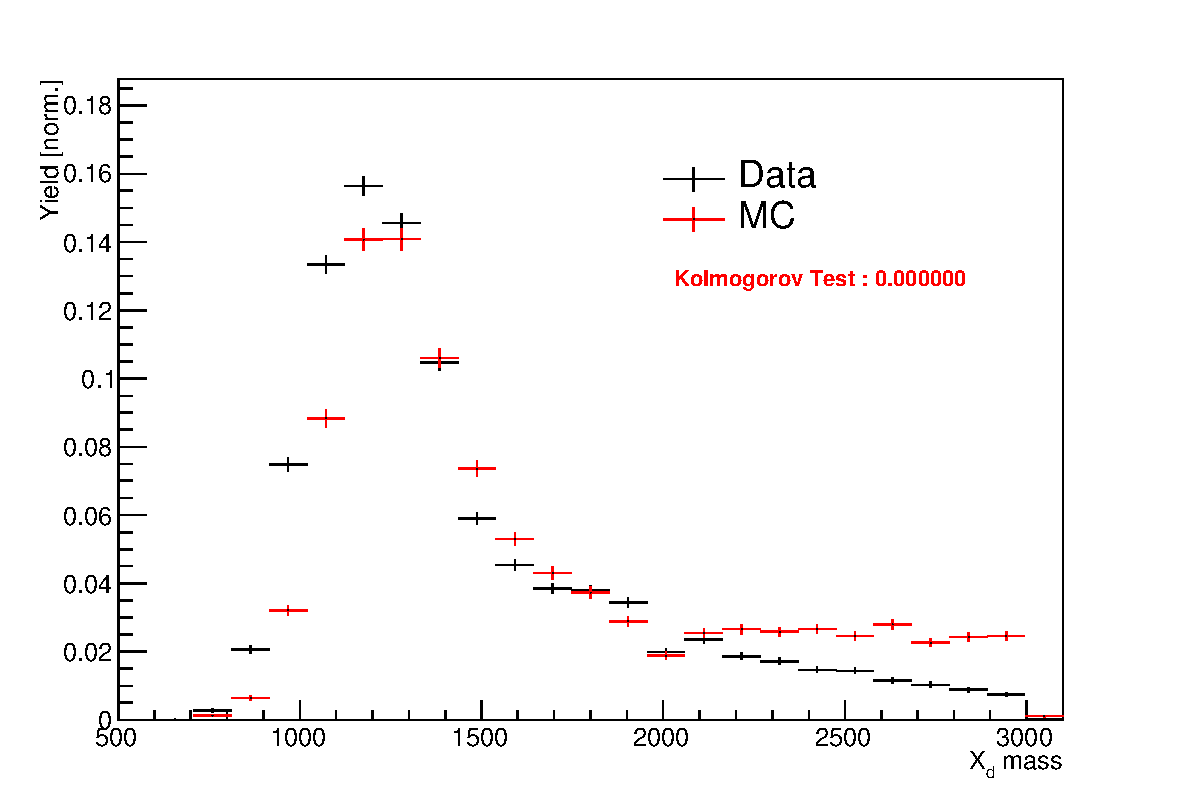
\includegraphics[height=6.cm,width=0.45\textwidth]{figs/Xd_Mass.pdf}
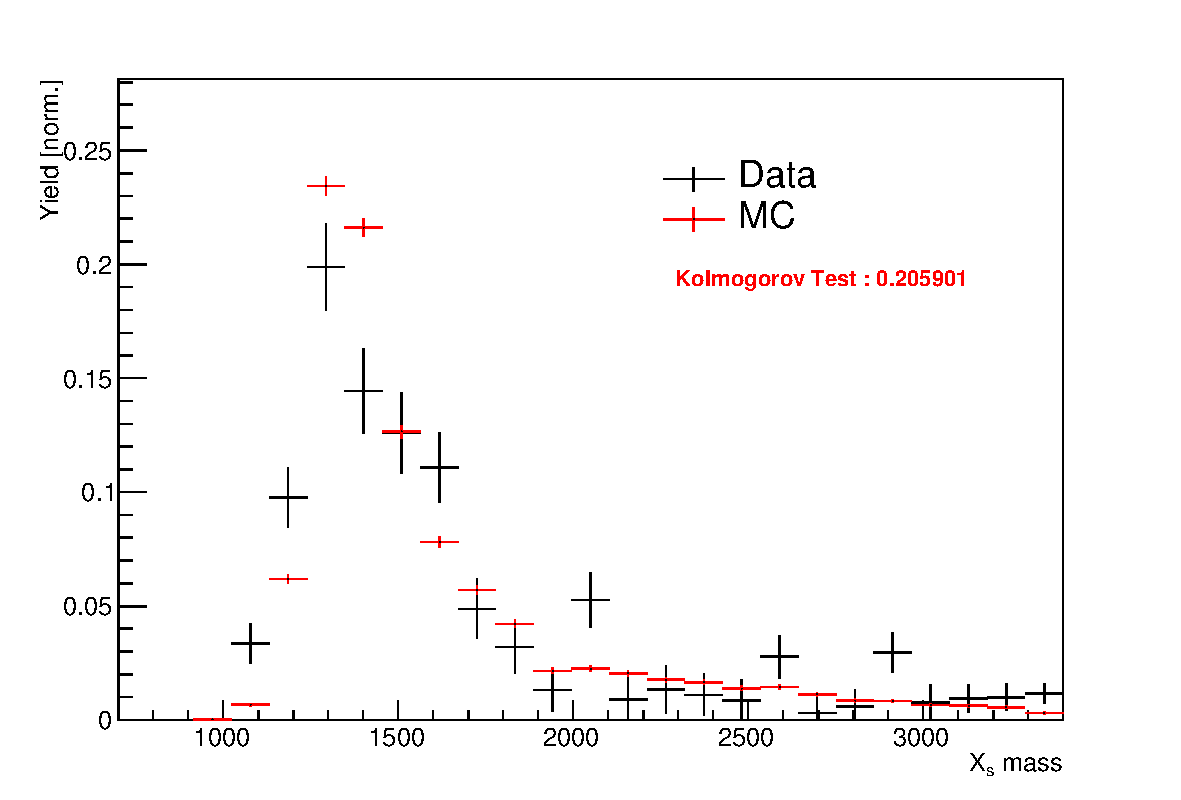
\includegraphics[height=6.cm,width=0.45\textwidth]{figs/Xs_Mass.pdf}
\caption{Comparison between (left) the $X_{d}$ invariant mass spectrum and (right) the $X_{s}$ invariant mass spectrum in (black) data and (red) simulation.}
\label{fig: XMasses}
\end{figure}


Applying the weights, we observe a 0.9 $\%$ variation in the selection efficiency of $\Bs\to\Ds\kaon\pion\pion$ candidates, while no significant change can be found in the efficiency of the 
$\Bs\to\Ds\pion\pion\pion$ channel. \newline  
We use the TISTOS method \cite{Tolk:1701134} to cross-check the simulated trigger efficiency on data. 
The efficiency of the used trigger lines on the signal decay (TOS) is calculated as $\epsilon_{TOS}=N_{TIS\&TOS}/N_{TIS}$, where $N_{TIS}$ is the number of signal events which are triggered independent of the signal decay (TIS) and
$N_{TIS\&TOS}$ denotes the number of events which are both triggered by signal decays and independently of signal decays.
We perform this cross-check using the full sample of $\Bs\to\Ds\pion\pion\pion$ decays and the corresponding MC.    
Figure \ref{fig: TriggerTISTOS} shows the trigger efficiencies for data and MC obtained by the TISTOS method, depending on the highest $\pt$ of the six final state particles, for the L0 and HLT1 trigger stage. 

\begin{figure}[h]
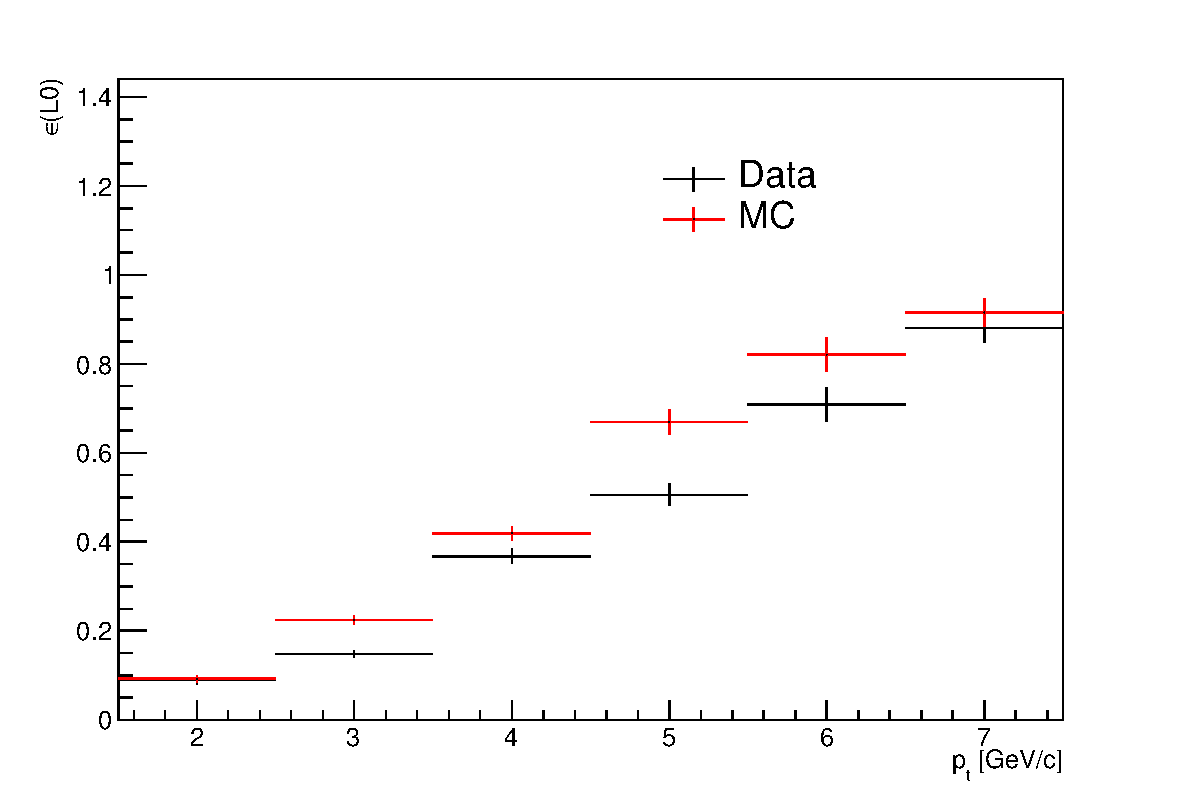
\includegraphics[height=6.cm,width=0.45\textwidth]{figs/L0_efficiency_comparison.pdf}
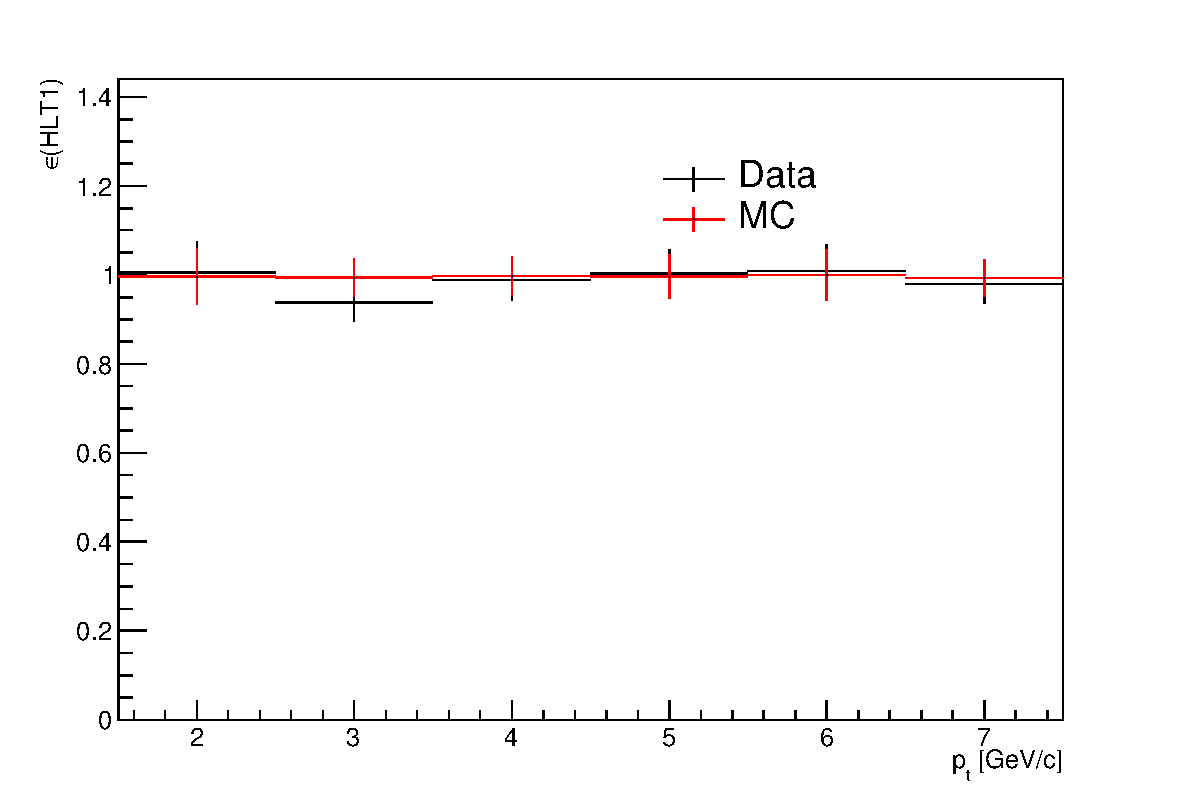
\includegraphics[height=6.cm,width=0.45\textwidth]{figs/HLT1_efficiency_comparison.pdf}
\caption{Trigger efficiencies of the (lef) L0 and (right) HLT1 trigger stage, determined by the TISTOS method on (black) data and (red) simulation.}
\label{fig: TriggerTISTOS}
\end{figure}

Although a systematic deviation between the trigger efficiency of the L0 stage in data and MC can be observed, 
this deviation appears in both the signal and normalization channel and cancels almost completely in every bin of $\pt$. A small systematic uncertainty of 0.1$\%$ remains.
The trigger efficiencies for the signal and normalization channel with respect to the HLT2 stage are compared on MC. 
An agreement, with deviations being well below the percent level, is observed and thus no systematic uncertainty is assigned to the HLT2 stage. \newline
Due to the different number of hadron types in the final state of the $\Bs\to\Ds\kaon\pion\pion$ and $\Bs\to\Ds\pion\pion\pion$ decay, a systematic uncertainty related to the tracking efficiency for both channels can arise.
To assess a potential difference in the tracking efficiency between the signal and normalization channel, 
we compare the ratio of the efficiency $\epsilon_{track}(data)/\epsilon_{track}(MC)$ in bins of track momentum $\ptot$ and pseudorapidity $\eta$ for both MC samples. 
Figure \ref{fig: TrackingTable} shows the ratio and its $\ptot$, $\eta$ dependence for 7 \& 8 $\tev$, using $\jpsi\to\mup\mun$ decays. 
This table is used to weight the simulated samples according to the pseudorapidity and total momentum of each track.

\begin{figure}[h]
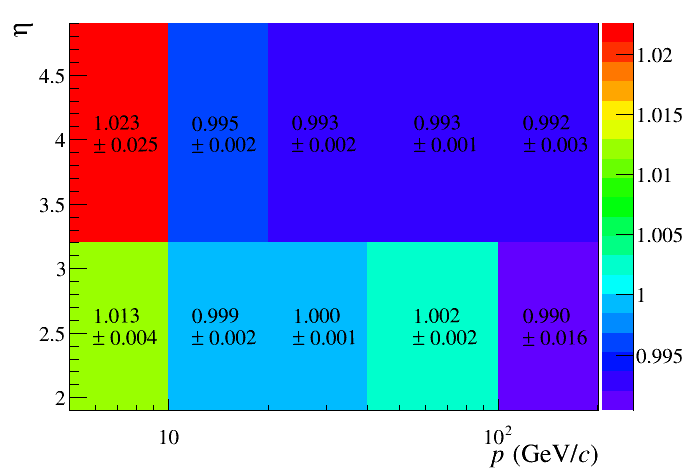
\includegraphics[height=6.cm,width=0.45\textwidth]{figs/ratio2011S20MC17.png}
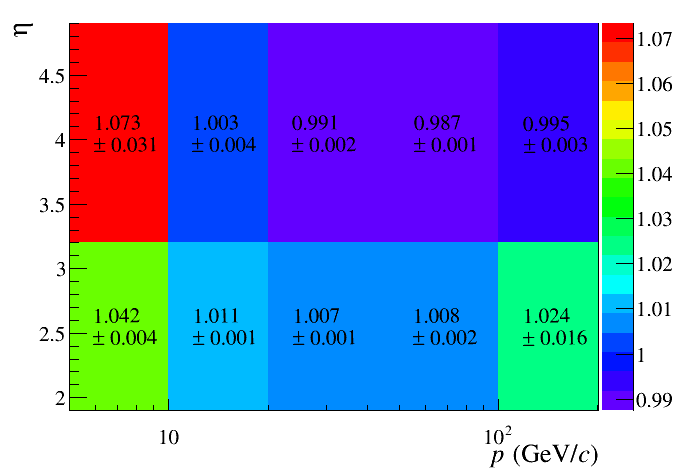
\includegraphics[height=6.cm,width=0.45\textwidth]{figs/ratio2012S20.png}
\caption{Tracking efficiency ratio for data over simulated events for (left) $\sqs = $ 7 $TeV$ and (right) $\sqs = $ 8 $TeV$.}
\label{fig: TrackingTable}
\end{figure}

A maximum deviation of $\Delta \epsilon_{track} =$ 1.5 $\%$ can be observed between the signal and normalization channel. Thus, this value is quoted as the systematical uncertainty due to the tracking efficiency.\newline
The uncertainty on the BDTG efficiency is determined by a fit to the $\Bs\to\Ds\pion\pion\pion$ invariant mass distribution with and without the BDTG cut. 
The maximum disagreement is found to be 1.9 $\%$ and is assigned as the uncertainty on the BDTG efficiency. \newline
The uncertainty due to the limited MC statistic is 1.3 $\%$. \newline
All systematic uncertainties are summarized in Table \ref{tab: systTab}. The quadratic sum of all contributions is 5.0 $\%$.  

\begin{table}[h!]
\centering
\begin{tabular}{l c}
Source  & Uncertainty on $\frac{\mathcal{B}(\Bs\to\Ds\kaon\pion\pion)}{\mathcal{B}(\Bs\to\Ds\pion\pion\pion)}$ [$\%$]\\
\hline
PID & 0.4 $\%$ \\
Mass fits & 4.0 $\%$\\
MC efficiency determination & 0.9 $\%$\\
Trigger efficiency & 0.1 $\%$\\
Tracking efficiency & 1.5 $\%$\\
BDTG efficiency & 1.9 $\%$ \\
MC statistics & 1.3 $\%$ \\
\hline
Total & 5.0 $\%$\\
\hline
\end{tabular}
\caption{Summary of considered systematic uncertainties on the branching ratio determination.}
\label{tab: systTab}
\end{table}
